\documentclass[11pt,a4paper]{report}
\usepackage[utf8]{inputenc} % For UTF-8 encoding
\usepackage[T1]{fontenc}    % For better font encoding
\usepackage[english]{babel} % For English language
\usepackage{graphicx}       % For including images
\usepackage{amsmath,amssymb}% For mathematical symbols
\usepackage{tikz}
\usetikzlibrary{shapes.geometric,arrows,positioning,calc,fit}
\usepackage{hyperref}       % For hyperlinks
\usepackage{geometry}       % For adjusting page margins
\usepackage{fancyhdr}       % For headers and footers
\usepackage{listings}       % For code listings
\usepackage{color}          % For color definitions
\usepackage{caption}        % For customizing captions
\usepackage{booktabs}       % For professional-looking tables
\usepackage{longtable}      % For tables that span multiple pages
\usepackage{float}          % For controlling float positions
\usepackage{array}          % For advanced table options
\usepackage{subfigure}
\usepackage{multirow}
\usepackage{multicol}
\geometry{margin=1in}
\setlength{\parskip}{0.5em}
\setlength{\parindent}{0em}
\usepackage[acronym]{glossaries}
\pagestyle{fancy}
\fancyhf{}
\lhead{Road Segmentation for AutoCar}
\rhead{\thepage}
\fancypagestyle{noNumber}{%
  \fancyhf{}
  \lhead{Road Segmentation for AutoCar}
  % clear all
  % no page number here
}
\makeatletter
\let\ps@plain\ps@fancy
\makeatother
\makeglossaries

\newacronym{kan}{KAN}{Kolmogorov-Arnold Network}
\newacronym{bnn}{BNN}{Binary Neural Network}
\newacronym{cnn}{CNN}{Convolutional Neural Network}
\newacronym{dl}{DL}{Deep Learning}
\newacronym{ml}{ML}{Machine Learning}
\newacronym{mlp}{MLP}{Multi-Layer Perceptron}
\newacronym{ukan}{UKAN}{U-shaped Kolmogorov-Arnold Network}
\newacronym{bika}{BiKA}{Binarized Kolmogorov-Arnold Network}
\newacronym{ste}{STE}{Straight-Through Estimator}
\newacronym{iou}{IoU}{Intersection over Union}
\newacronym{bn}{BN}{Batch Normalisation}
\newacronym{cv}{CV}{Computer Vision}
\newacronym{ai}{AI}{Artificial Intelligence}
\renewcommand{\listfigurename}{LIST OF FIGURES}
\renewcommand{\listtablename}{LIST OF TABLES}



\begin{document}
\pagenumbering{arabic}

\begin{titlepage}
\begin{tikzpicture}[remember picture, overlay]
  \draw[thick] ($(current page.north west) + (2cm, -2cm)$) rectangle ($(current page.south east) + (-2cm, 2cm)$);
\end{tikzpicture}

\begin{center}
    {\small 
    UNIVERSITY OF SCIENCE AND TECHNOLOGY OF HANOI \\
    \textbf{DEPARTMENT OF INFORMATION AND COMMUNICATION TECHNOLOGY} 
    } \\[1.5cm]

    % USTH Logo
    
\includegraphics[width=0.45\linewidth]{images/usth.png} \\[1.5cm]

    {\Huge \textbf{MASTER THESIS}}\\[1.5cm]

    {\Large By} \\[0.5cm]
    {\Large Dao Xuan Quy - 2440053} \\[1cm]

    {\Large Title:} \\[0.5cm]
    {\huge \textbf{\uppercase{Road Segmentation for AutoCar}} \\[0.5cm] 
    \textbf{\uppercase{Networks}}} \\[2cm]
    
    {\Large
    \begin{tabular}{rl}
        Supervisor: & Dr. Nghiem Thi Phuong \\
    \end{tabular}
    } \\[3cm]

    {\Large \textbf{Hanoi, August -- 2026}}
\end{center}
\end{titlepage}

\clearpage
\thispagestyle{empty}
To whom it may concern,

I, Nghiem Thi Phuong, certify that the internship report of Mr. Dao Xuan Quy is qualified to be presented in the Internship Jury 2025-2026.

Hanoi, August 2026

Supervisor's signature\\
\\
\\
\\
\\

Nghiem Thi Phuong



\clearpage
\pagenumbering{Roman}  % Start Roman page numbering
\setcounter{page}{1}   % Start from I


\tableofcontents

\addcontentsline{toc}{chapter}{Content}
\listoffigures
\addcontentsline{toc}{chapter}{List of Figures}
\clearpage

% List of Tables
\listoftables
\addcontentsline{toc}{chapter}{List of Table}

\printglossary[type=\acronymtype,title=List of Abbreviations]
\addcontentsline{toc}{chapter}{List of Abbreviations}




\newpage
\chapter*{Declaration}
\addcontentsline{toc}{chapter}{Declaration}
I hereby, Dao Xuan Quy, declare that my thesis represents my own work after doing an internship at USTH ICTLAB, University of Science and Technology of Hanoi.

I have read the University's internship guidelines. In the case of plagiarism appearing in my thesis, I accept responsibility for the conduct of the procedures in accordance with the
University's Committee.

Hanoi, August 2026\\

Signature\\
\\
\\
\\
\\
Dao Xuan  Quy


\chapter*{Acknowledgements}
\addcontentsline{toc}{chapter}{Acknowledgements}
 I would like to express my sincere gratitude to Dr. Nghiem Thi Phuong and A.Prof. Tran Giang Son for they exceptional guidance and support throughout this project. I am also grateful to USTH for providing me with the computational resources needed to complete this research, and to the open-source communities behind the KAN, BiKA and U-KAN projects for providing foundational implementations.

\chapter*{Abstract}
\addcontentsline{toc}{chapter}{Abstract}

Semantic segmentation is a critical component of autonomous driving perception, requiring both high accuracy and low latency for real-time deployment. Traditional segmentation networks based on U-Net \cite{ronneberger2015unet},  and Transformer architectures rely on Multi-Layer Perceptrons (MLPs) with fixed activation functions, limiting their representational flexibility. On the other hand, lightweight models often suffer from accuracy loss when handling more complicated classes.
In this thesis, we study and implement two novel approaches that integrate Kolmogorov-Arnold Networks (KANs) into segmentation architectures for road segmentation. The main contributions of this thesis include:
\begin{itemize}
    \item Optimizing and Evaluating U-KAN (UKAN), a U-Net style segmentation network that replaces standard MLP layers with KAN layers using learnable activation functions, including multiple KAN variants: FasterKAN (RSWAf basis) , ReLU-KAN, HardSwish-KAN, PWLO-KAN, and TeLU-KAN.
    \item Implementing and evaluating BiKA (Binarized KAN), a novel architecture that combines the KAN philosophy of per-connection learnable activations with Binary Neural Network (BNN) techniques, achieving extreme compression through 1-bit binarized weights and activations.
    \item Improving BiKA \cite{liu2026bika} GPU performance by apply GPU optimization methods to the official implementation
    \item Benchmarking both architectures against standard baselines in terms of segmentation accuracy (mIoU, Dice), model size, and inference throughput with two distinct problems: Segment Everything (20 classes) and Segment the drivable area only (2 classes)
  \end{itemize}

The experimental results demonstrate that KAN-based architectures successfully achieve a highly accurate segmentation results for multi-class segmentation with UKAN architectures, and retain acceptable accuracy while perform extremely fast with BiKA implementations.

\textbf{Keywords:} Kolmogorov-Arnold Networks, Semantic Segmentation, Binary Neural Networks, Road Segmentation, U-Net, Edge Deployment.

\clearpage
\pagenumbering{arabic}
\setcounter{page}{1}
\chapter{Introduction}
\section{Context and motivation}
\label{sec:context}
\subsection{Context}
Semantic segmentation, the task of assigning a class label to every pixel in an image, is a foundational capability for autonomous driving perception systems. Accurate road segmentation enables autonomous vehicles to identify drivable surfaces, lane boundaries, sidewalks, and other critical scene elements in real time. The evolution of segmentation architectures has progressed from early fully convolutional networks (FCN)~\cite{long2015fcn} to the U-Net encoder-decoder architecture~\cite{ronneberger2015unet}, and more recently to Transformer-based models such as SegFormer~\cite{xie2021segformer}, Swin-UNet~\cite{cao2022swinunet} and Segment Anything~\cite{kirillov2023segment}.

However, all of these architectures share a fundamental design choice inherited from Multi-Layer Perceptrons (MLPs): they place fixed, pre-defined activation functions (e.g., ReLU, GELU) at the \emph{nodes} of the network, while the \emph{edges} (connections) carry only learnable linear weights,. The Kolmogorov-Arnold Representation Theorem~\cite{kolmogorov1957, arnold2009} suggests an alternative: replace every linear weight with a non-linear activation functions on the \emph{edges} themselves, allowing the network to learn both the weights and the optimal activation shape for each connection, which as a results, achieve better accuracy and interpretability. This principle forms the foundation of Kolmogorov-Arnold Networks (KANs)~\cite{liu2024kan}.

In the Sematic Segmentation contenxt, recent work has demonstrated the potential of KAN-based architectures in medical image segmentation~\cite{li2024ukan}. On the other hand,  KAN application to road scene segmentation and their compatibility with extreme model compression techniques such as Binary Neural Networks (BNNs)~\cite{qin2020bireal, liu2020reactnet} remain largely unexplored.

\subsection{Problem Statement}
Deploying segmentation models on autonomous vehicles poses two competing requirements. First, the model must achieve high segmentation accuracy to to ensures safeness to vehicles and the passengers. Second, since the car \textbf{sees} the environment throught a camera, the model itself have to be capable of processing a large amount of frames per second; therefore, require low latency, small model size, and minimal memory bandwidth.

Standard full-precision segmentation networks (32-bit floating point) achieve high accuracy but require significant computational resources. Binary Neural Networks (BNNs) offer extreme compression by quantizing both weights and activations to 1-bit representations, but they suffer from severe accuracy degradation due to the limited expressiveness of the sign function used for binarization. The central challenge addressed in this thesis is: \emph{Can the KAN solve the accuracy loss in efficient, binarized networks, while preserving their computational efficiency advantages?}

\subsection{Motivation}
This research is motivated by the need to bridge the gap between expressive, high-accuracy segmentation models and the efficient model real-time performance. We perform two approaches: UKAN for full-precision KAN-augmented segmentation and BiKA for binarized KAN convolutions—we aim to observe how KAN integration affects the accuracy-efficiency for road segmentation. 

\section{Related Work}
\label{sec:related_work}
The development of semantic segmentation architectures has grown significant for the last decade. In 2015, Long et al.~\cite{long2015fcn} introduced Fully Convolutional Networks (FCN), demonstrating that classification CNNs could be adapted for dense prediction. Ronneberger et al.~\cite{ronneberger2015unet} proposed U-Net, whose symmetric encoder-decoder architecture with skip connections became the dominant standard for biomedical and subsequently autonomous driving segmentation.

Modern segmentation architectures have increasingly adopt attention mechanisms. SegFormer~\cite{xie2021segformer} introduced a hierarchical Transformer encoder with efficient self-attention, while Swin-UNet~\cite{cao2022swinunet} adapted the shifted-window Transformer for U-shaped segmentation. DeepLabV3+~\cite{chen2018deeplabv3plus} combined atrous spatial pyramid pooling with encoder-decoder structures to capture multi-scale context.

In parallel, the Kolmogorov-Arnold Network (KAN) was proposed by Liu et al.~\cite{liu2024kan} as an alternative to MLPs, placing learnable activation functions on edges rather than nodes. Li et al.~\cite{li2024ukan} subsequently demonstrated U-KAN, integrating KAN layers into the U-Net bottleneck for medical image segmentation. FasterKAN~\cite{fasterkan2024} addressed the computational overhead of the original B-spline KAN implementation by replacing B-splines with Reflectional Switch Activation Functions (RSWAf).

On the model compression side, Binary Neural Networks (BNNs) were first formalized by Hubara et al.~\cite{hubara2016binarized}, who demonstrated the feasibility of training deep networks with weights and activations constrained to $+1$ and $-1$. Subsequent works like XNOR-Net~\cite{rastegari2016xnor} and Bi-Real Net~\cite{qin2020bireal} advanced BNNs by introducing real-valued skip connections to stabilize binary training. ReActNet~\cite{liu2020reactnet} further improved BNN accuracy through learnable activation shifts (RPReLU), while IR-Net~\cite{qin2020irnet} proposed Libra-PB for balanced weight binarization, and AdaBin~\cite{tu2022adabin} introduced learnable per-channel output scaling. Extending these principles to dense prediction tasks, Group-Net~\cite{zhuang2019structured} demonstrated that structured binary networks, which dvide operations into multiple homogeneous binary branches, can successfully maintain the rich contextual information required for accurate semantic segmentation.

Our work builds upon these foundations by: (1) adapting U-KAN for road segmentation with multiple efficient KAN variants, and (2) proposing BiKA, which combines the KAN per-connection activation idea with state-of-the-art BNN techniques for extreme efficiency.

\section{Thesis Objective} 
\label{sec: obj}
The primary objective of this thesis is to implement, evaluate, and compare two KAN-based segmentation architectures for road segmentation problem. Specifically, we aim to: 

\begin{itemize}
    \item Adapt the U-KAN architecture for road segmentation on the BDD100K dataset, exploring multiple KAN linear variants (FasterKAN, ReLU-KAN, HardSwish-KAN, PWLO-KAN, TeLU-KAN) to assess their impact on segmentation accuracy and inference speed.
    \item Design and implement BiKASegNet, a binarized segmentation network that applies the KAN algorithm through per-connection binary thresholds to achieve extreme model compression while retaining acceptable accuracy.
    \item Benchmark both architectures against standard baseline models in terms of segmentation quality (mIoU, Dice), model size, and inference speed on CUDA platforms.
      
\end{itemize}
      
\section{Thesis Structure}
\label{sec: structure}
The remainder of this thesis is structured as follows:
\begin{itemize}
    \item \textbf{Chapter 1} introduces the context, problem statement, related work, and objectives of this research.
    \item \textbf{Chapter 2} discusses the technical background of Kolmogorov-Arnold Networks, the U-Net segmentation, Binary Neural Networks, and the KAN variant implementations.
    \item \textbf{Chapter 3} explains the methodology, including the UKAN architecture, KAN layer integration, the BiKA binarized segmentation network design.
    \item \textbf{Chapter 4} describes the experimental setup, dataset preparation, training procedures, and performance evaluation of both architectures.
    \item \textbf{Chapter 5} summarizes the content of this thesis and proposes future developments of research.

\end{itemize}



\chapter{Background}
\label{ch:background}

This chapter introduces the foundational knowledge that are used to implement KAN-based segmentation networks. These include Kolmogorov-Arnold Networks (KANs), Binary Neural Networks (BNNs), and Binarized Kolmogorov-Arnold Networks (BiKA) concept which sucessfully combine the two architectures. 

Binary Neural Networks (BNNs) address the hardware constraints of deep learning by pushing model quantization to its absolute theoretical limit. In a BNN, both the network weights and the intermediate feature activations are constrained to 1-bit representations, typically $\{-1, +1\}$, utilizing the sign function. This severe quantization completely eliminates the need for expensive floating-point multiply-accumulate (MAC) operations. Instead, convolutions and dense layers can be executed using highly efficient bitwise XNOR and popcount operations, drastically reducing memory bandwidth and latency on edge devices like FPGAs and embedded GPUs. Despite these immense computational advantages, the extreme information loss induced by binarizing continuous variables natively limits the expressiveness of BNNs. They often suffer from accuracy compared to full-precision networks and require specialized training methodologies, such as the Straight-Through Estimator (STE) and dense skip connections, to maintain stable gradient flow during backpropagation.

Bridging the gap between the high representational capacity of KANs and the extreme hardware efficiency of BNNs, the Binarized Kolmogorov-Arnold Network (BiKA) introduces a novel paradigm for edge-deployed neural networks. While traditional KANs employ computationally expensive continuous splines and standard BNNs rely on uniform binarization, BiKA replaces the continuous edge functions of KANs with learnable, binary step functions parameterized by individualized connection thresholds. By assigning a unique, learnable bias threshold to every single synapse before binarization, BiKA faithfully implements the KAN philosophy of per-connection activations without requiring floating-point arithmetic during inference. Compared to KANs, BiKA sacrifices the smooth continuity of spline functions to achieve a completely multiply-free computational graph. Compared to traditional BNNs, BiKA achieves significantly higher expressiveness without adding computational complexity by shifting the learning capacity from continuous weight magnitudes to highly localized spatial thresholds. This synthesis provides a highly effective balance, delivering KAN-inspired accuracy within the strict power and resource budgets of binary architectures.


\section{Kolmogorov-Arnold Networks}
\label{sec:kan_background}

The Kolmogorov-Arnold Representation Theorem~\cite{kolmogorov1957, arnold2009} states that any multivariate continuous function $f: [0,1]^n \rightarrow \mathbb{R}$ can be represented as a finite composition of continuous functions of a single variable and the binary operation of addition:
\begin{equation}
    f(x_1, \dots, x_n) = \sum_{q=0}^{2n} \Phi_q \left( \sum_{p=1}^{n} \phi_{q,p}(x_p) \right)
\end{equation}
where $\phi_{q,p}: [0,1] \rightarrow \mathbb{R}$ are univariate inner functions and $\Phi_q: \mathbb{R} \rightarrow \mathbb{R}$ are outer functions. This theorem guarantees the existence of such a representation but does not prescribe how to learn it.

Kolmogorov-Arnold Networks (KANs) \cite{liu2024kan} have been proposed as a novel approach to improve traditional Multi-Layer Perceptrons (MLPs) accuracy, inspired by the Kolmogorov-Arnold representation theorem. In a standard MLP, the network learns fixed scalar weights on its connections (edges) and applies pre-defined, fixed non-linear activation functions (such as ReLU or sigmoid) at its neurons (nodes). KANs invert this principle by placing learnable, non-linear activation functions directly on the network edges, while the nodes simply sum the incoming signals. The key different between KANs and traditional MLPs is illustrated in Figure~\ref{fig:kan_vs_mlp}.

\begin{figure}[H]
\centering
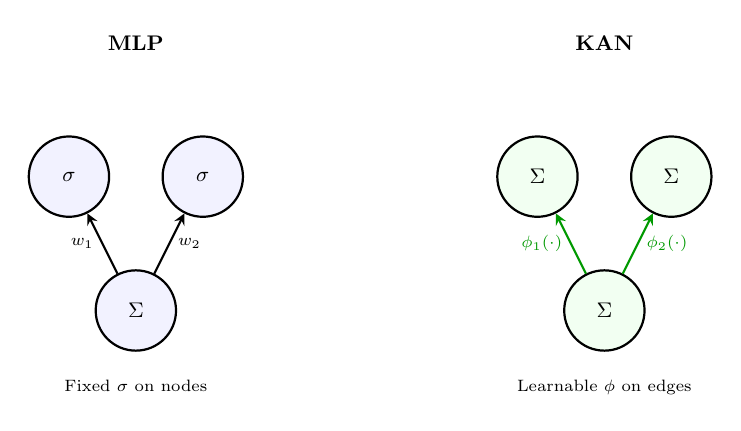
\begin{tikzpicture}[>=stealth, thick, scale=0.85, transform shape]
    \tikzset{
        neuron/.style={draw, circle, minimum size=1.2cm, fill=blue!5, font=\small},
        kanneuron/.style={draw, circle, minimum size=1.2cm, fill=green!5, font=\small},
        label/.style={font=\small\bfseries}
    }
    
    % MLP side
    \node[label] at (-3.5, 4) {MLP};
    \node[neuron] (m1) at (-4.5, 2) {$\sigma$};
    \node[neuron] (m2) at (-2.5, 2) {$\sigma$};
    \node[neuron] (m3) at (-3.5, 0) {$\Sigma$};
    
    \draw[->, thick] (m3) -- node[left, font=\scriptsize] {$w_1$} (m1);
    \draw[->, thick] (m3) -- node[right, font=\scriptsize] {$w_2$} (m2);
    \node[font=\scriptsize, below=0.3cm of m3] {Fixed $\sigma$ on nodes};
    
    % KAN side
    \node[label] at (3.5, 4) {KAN};
    \node[kanneuron] (k1) at (2.5, 2) {$\Sigma$};
    \node[kanneuron] (k2) at (4.5, 2) {$\Sigma$};
    \node[kanneuron] (k3) at (3.5, 0) {$\Sigma$};
    
    \draw[->, thick, green!60!black] (k3) -- node[left, font=\scriptsize] {$\phi_1(\cdot)$} (k1);
    \draw[->, thick, green!60!black] (k3) -- node[right, font=\scriptsize] {$\phi_2(\cdot)$} (k2);
    \node[font=\scriptsize, below=0.3cm of k3] {Learnable $\phi$ on edges};
\end{tikzpicture}
\caption{MLP vs KAN~\cite{liu2024kan}.}
\label{fig:kan_vs_mlp}
\end{figure}

In an MLP, each neuron computes:
\begin{equation}
    y_j = \sigma\left(\sum_i w_{ij} x_i + b_j \right)
\end{equation}
where $\sigma$ is a fixed activation function (e.g., ReLU) and $w_{ij}$ are learnable scalar weights. In a KAN, each node simply sums its incoming signals, and each edge applies a learnable univariate function:
\begin{equation}
    y_j = \sum_i \phi_{ij}(x_i)
\end{equation}
where $\phi_{ij}: \mathbb{R} \rightarrow \mathbb{R}$ are learnable activation functions parameterized as spline functions. This places the representational power on the edges rather than the nodes.

\subsection{Original KAN Implementation with B-Splines}
In the original KAN~\cite{liu2024kan}, each edge activation $\phi_{ij}$ is parameterized as a B-spline:
\begin{equation}
    \phi_{ij}(x) = w_b \cdot \text{SiLU}(x) + w_s \cdot \text{spline}(x)
\end{equation}
where $\text{SiLU}(x) = x \cdot \sigma(x)$ is a base activation, and $\text{spline}(x) = \sum_k c_k B_k(x)$ is a linear combination of B-spline basis functions $B_k$ with learnable coefficients $c_k$. The B-spline is defined over a grid of knot points $\{t_0, t_1, \dots, t_G\}$ spanning the input domain.

As a trade-off to the extra information captured, B-spline evaluation requires iterative recursion over the grid, resulting in $\mathcal{O}(G \cdot k)$ operations per activation (where $G$ is the grid size and $k$ is the spline order), making the original KAN impractical for high-throughput vision tasks. This is the main problem that we address in this thesis.


\label{sec:kan_variants}
\subsection{Optimized KAN networks}
To overcome the computational bottleneck of B-splines, several efficient KAN linear replacements have been proposed. Each variant maintains the KAN philosophy of learning activation functions on edges but uses faster basis functions.

\textbf{FastKAN~\cite{li2024fastkan}} reframes Kolmogorov-Arnold Networks through the lens of Radial Basis Function (RBF) networks. It replaces the computationally intensive 3rd-order B-splines with Gaussian RBF basis functions defined over a uniform grid of center points $\{g_0, g_1, \dots, g_{G-1}\}$:
\begin{equation}
    \psi_k(x) = \exp\left( -\left(\frac{x - g_k}{\gamma}\right)^2 \right)
\end{equation}
where $\gamma > 0$ controls the bandwidth of the Gaussian basis functions. Each univariate activation function on edge $(i, j)$ is constructed as a linear combination of these Gaussian RBFs alongside a base linear projection:
\begin{equation}
    \phi_{ij}(x) = w_{\text{base}} \cdot \text{SiLU}(x) + \sum_{k=0}^{G-1} c_{k,ij} \cdot \psi_k(x)
\end{equation}
where $c_{k,ij}$ are learnable expansion coefficients. By avoiding the iterative grid recursion required by B-splines, FastKAN computes basis evaluations in parallel via matrix multiplication, enabling execution speed comparable to standard MLPs while retaining KAN's edge-centric non-linear expressiveness.

\textbf{PowerMLP~\cite{qiu2024powermlp}} addresses KAN's training latency bottleneck by reformulating the edge-centric spline activation functions into non-iterative power-basis expansions. Instead of evaluating localized grid splines or RBFs, PowerMLP approximates each non-linear univariate edge function $\phi(x)$ using a polynomial power-series expansion of order $K$:
\begin{equation}
    \phi(x) = \sum_{k=1}^{K} w_k \cdot \sigma(x)^k
\end{equation}
where $\sigma(x)$ is a base non-linear activation function (such as SiLU or GELU), and $w_k$ are learnable scalar weights associated with each power $k$. The layer output for an input vector $\mathbf{x} \in \mathbb{R}^{d_{\text{in}}}$ is computed via vectorized elementwise powers and linear projections:
\begin{equation}
    y = \sum_{k=1}^{K} \mathbf{W}_k \left( \sigma(\mathbf{x})^k \right)
\end{equation}
where $\mathbf{W}_k \in \mathbb{R}^{d_{\text{out}} \times d_{\text{in}}}$ are standard weight matrices. Because power calculations ($\mathbf{x}^k$) are fully parallelizable and require no grid lookups or localized indexing, PowerMLP drastically reduces FLOPs and achieves up to $40\times$ faster training speed than standard B-spline KANs, combining MLP-like execution throughput with KAN-level non-linear representational power.

\textbf{FasterKAN~\cite{fasterkan2024}} replaces B-splines with the Reflectional Switch Activation Function (RSWAf). Given a set of grid points $\{g_0, g_1, \dots, g_{G-1}\}$ uniformly spanning $[g_{\min}, g_{\max}]$ and an inverse denominator parameter $\beta$, the basis function is:
\begin{equation}
    r_k(x) = 1 - \tanh^2\left((x - g_k) \cdot \beta\right)
\end{equation}
Each basis function $r_k$ produces a smooth, localized bump centred at grid point $g_k$. The output of a FasterKAN linear layer with input dimension $d_{\text{in}}$ and output dimension $d_{\text{out}}$ is:
\begin{equation}
    y = \mathbf{W}_s \cdot \text{vec}\left(\{r_k(x_i)\}_{k=0,\dots,G-1}^{i=1,\dots,d_{\text{in}}}\right)
\end{equation}
where $\mathbf{W}_s \in \mathbb{R}^{d_{\text{out}} \times (d_{\text{in}} \cdot G)}$ is a learnable spline projection matrix, and $\text{vec}(\cdot)$ concatenates all basis evaluations into a single vector. The input is first normalised via LayerNorm. A custom CUDA kernel computes the forward and backward passes of the RSWAf function, achieving significant speedups over the B-spline implementation.


\textbf{ReLU-KAN~\cite{qiu2024relukan}} replaces the smooth basis with a piecewise-linear function using ReLU:
\begin{equation}
    \psi_k(x) = \text{ReLU}(x - g_k) = \max(0, x - g_k)
\end{equation}
This produces a basis of shifted ramp functions. The output is computed as:
\begin{equation}
    y = \mathbf{W} \cdot \text{vec}\left(\{\psi_k(x_i)\}_{k,i}\right)
\end{equation}
ReLU-KAN achieves maximal inference speed due to the trivial cost of ReLU evaluation, but trades off smoothness for speed.

With the same policy proposed by FasterKAN \cite{fasterkan2024} and ReLU-KAN \cite{qiu2024relukan}, we decide to perform evaluation with more activation functions which have a lower computational complexity compared original KAN to find out the optimal point between efficiency and accuracy.
\begin{itemize}

  \item HardSwish~\cite{howard2019searching} is defined mathematically as:
    \begin{equation}
        \text{HardSwish}(x) = x \cdot \frac{\text{ReLU6}(x + 3)}{6}
    \end{equation}
    It serves as a computationally efficient, piecewise-linear approximation of the smooth Swish activation function ($x \cdot \sigma(x)$). By replacing the continuous exponential function in Sigmoid with a bounded linear ramp ($\text{ReLU6}(x) = \min(\max(0, x), 6)$), HardSwish enforces piecewise linearity across the input domain. For $x \le -3$, the output is identically 0; for $x \ge 3$, the function becomes purely linear ($f(x) = x$). In the intermediate region $[-3, 3]$, it forms a quadratic-like piecewise linear transition. This piecewise linear structure eliminates expensive transcendental operations while maintaining gradient stability for deep networks.

  \item The Hyperbolic Tangent Exponential Linear Unit (TeLU)~\cite{fernandez2024telu} is formulated as:
    \begin{equation}
        \text{TeLU}(x) = x \cdot \tanh(\exp(x))
    \end{equation}
    TeLU is designed to combine the fast convergence of linear activations with the smooth non-linear saturation of exponential units. In the active positive domain ($x > 0$), $\exp(x)$ increases rapidly, driving $\tanh(\exp(x)) \approx 1$. Consequently, $\text{TeLU}(x) \approx x$, displaying strong positive-region linearity (identity mapping) that allows gradients to flow unattenuated. In the negative domain ($x < 0$), the smooth decay of $\tanh(\exp(x))$ prevents dying activations while bounding negative values, maintaining a seamless transition between linear and non-linear regimes.

  \item Piecewise Linear Optimisation (PWLO)~\cite{schoots2025relating} approximates non-linear continuous functions by partitioning the input domain $[g_{\min}, g_{\max}]$ into $G$ sub-intervals $[g_k, g_{k+1})$ and assigning a localized linear affine transformation to each segment:
  \begin{equation}
      f(x) = a_k \cdot x + b_k, \quad x \in [g_k, g_{k+1})
  \end{equation}
  where $a_k$ and $b_k$ denote the slope and offset of the $k$-th segment. PWLO explicitly enforces local linearity within each interval. By converting complex non-linear functions into a composition of linear segments, PWLO enables high-throughput execution using simple linear primitives (multiply-accumulate or shift-and-add) on edge acceleration hardware.
\end{itemize}
\section{U-Net Segmentation Architecture}
\label{sec:unet}
U-Net~\cite{ronneberger2015unet} established the symmetric encoder-decoder architecture with skip connections as the standard for dense prediction tasks. The encoder progressively downsamples the input through convolutional blocks and pooling operations, extracting increasingly abstract feature representations. The decoder upsamples these features back to the original resolution, with skip connections from corresponding encoder stages providing fine-grained spatial detail.

Each encoder stage consists of a double convolution block:
\begin{equation}
    \text{ConvLayer}(x) = \text{ReLU}(\text{BN}(\text{Conv}_{3\times3}(\text{ReLU}(\text{BN}(\text{Conv}_{3\times3}(x))))))
\end{equation}
followed by $2\times2$ max pooling for spatial downsampling. The decoder mirrors this structure using bilinear upsampling and concatenation (or addition) with encoder skip connections, as illustrated in Figure~\ref{fig:unet_arch}.

\begin{figure}[H]
\centering
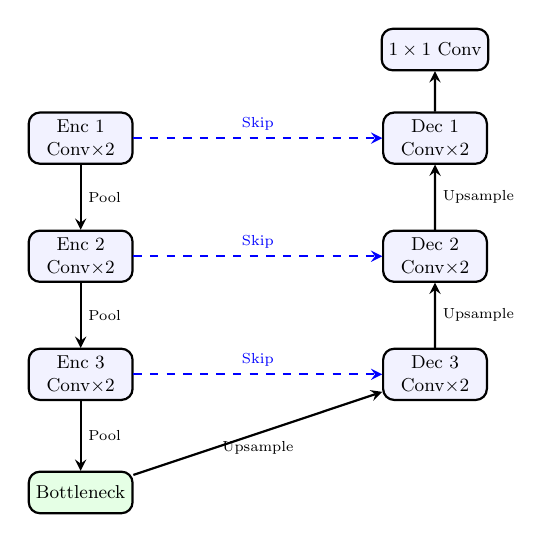
\begin{tikzpicture}[>=stealth, thick, scale=0.75, transform shape]
    \tikzset{
        block/.style={draw, fill=blue!5, rectangle, minimum height=2em, minimum width=5em, rounded corners, align=center, font=\small},
        kanblock/.style={draw, fill=green!10, rectangle, minimum height=2em, minimum width=5em, rounded corners, align=center, font=\small},
        line/.style={draw, ->, >=stealth, thick}
    }
    % Encoder
    \node[block] (e1) at (0, 0) {Enc 1\\Conv$\times$2};
    \node[block] (e2) at (0, -2) {Enc 2\\Conv$\times$2};
    \node[block] (e3) at (0, -4) {Enc 3\\Conv$\times$2};
    \node[kanblock] (b) at (0, -6) {Bottleneck};
    
    % Decoder
    \node[block] (d3) at (6, -4) {Dec 3\\Conv$\times$2};
    \node[block] (d2) at (6, -2) {Dec 2\\Conv$\times$2};
    \node[block] (d1) at (6, 0) {Dec 1\\Conv$\times$2};
    \node[block] (out) at (6, 1.5) {$1\times1$ Conv};
    
    % Encoder connections
    \path[line] (e1) -- node[right, font=\scriptsize] {Pool} (e2);
    \path[line] (e2) -- node[right, font=\scriptsize] {Pool} (e3);
    \path[line] (e3) -- node[right, font=\scriptsize] {Pool} (b);
    
    % Decoder connections
    \path[line] (b) -- node[below, font=\scriptsize] {Upsample} (d3);
    \path[line] (d3) -- node[right, font=\scriptsize] {Upsample} (d2);
    \path[line] (d2) -- node[right, font=\scriptsize] {Upsample} (d1);
    \path[line] (d1) -- (out);
    
    % Skip connections
    \draw[line, dashed, blue] (e3.east) -- node[above, font=\scriptsize] {Skip} (d3.west);
    \draw[line, dashed, blue] (e2.east) -- node[above, font=\scriptsize] {Skip} (d2.west);
    \draw[line, dashed, blue] (e1.east) -- node[above, font=\scriptsize] {Skip} (d1.west);
\end{tikzpicture}
\caption{Standard U-Net encoder-decoder architecture with skip connections~\cite{ronneberger2015unet}.}
\label{fig:unet_arch}
\end{figure}


\section{Binary Neural Networks}
\label{sec:bnn}
Binary Neural Networks (BNNs) address the hardware constraints of deep learning models by simplify the mathematics back to Binary operations. The binarization function for weights is:
\begin{equation}
    w_b = \text{sign}(w) = \begin{cases} +1 & \text{if } w \geq 0 \\ -1 & \text{otherwise} \end{cases}
\end{equation}
and similarly for activations: $x_b = \text{sign}(x)$. This allows the multiply-accumulate operations in convolutions to be replaced by XNOR and popcount operations:
\begin{equation}
    w_b \cdot x_b = \text{XNOR}(w_b, x_b), \quad \sum_i w_{b,i} \cdot x_{b,i} = \text{popcount}(\text{XNOR}(\mathbf{w}_b, \mathbf{x}_b))
\end{equation}
achieving up to $\sim$58$\times$ theoretical speedup and $\sim$32$\times$ memory reduction compared to full-precision networks~\cite{rastegari2016xnor}.
In a BNN, both the network weights and the intermediate feature activations are constrained to 1-bit representations, typically $\{-1, +1\}$, utilizing the sign function. This mehod completely eliminates the need for expensive floating-point multiply-accumulate (MAC) operations. Instead, convolutions and dense layers can be executed using highly efficient bitwise XNOR and popcount operations, drastically reducing memory bandwidth and latency on edge devices. Despite these immense computational advantages, the extreme information loss induced by binarizing continuous variables natively limits the expressiveness of BNNs. They often suffer from accuracy compared to full-precision networks and require specialized training methodologies, such as the Straight-Through Estimator (STE) and dense skip connections, to maintain stable gradient flow during backpropagation.


\subsection{Straight-Through Estimator (STE)}
The sign function has zero gradient almost everywhere, making direct backpropagation impossible. Bengio et al.~\cite{bengio2013ste} proposed the Straight-Through Estimator (STE), which approximates the gradient of the sign function as:
\begin{equation}
    \frac{\partial \mathcal{L}}{\partial w} \approx \frac{\partial \mathcal{L}}{\partial w_b} \cdot \mathbf{1}_{|w| \leq 1}
\end{equation}
where the gradient is passed through unchanged within the clipping window $[-1, 1]$ and zeroed outside. This enables training of binary networks with standard gradient-based optimisers.

\subsection{Key BNN Techniques}
Several techniques have been developed to improve the accuracy of BNNs:

\subsubsection{Bi-Real Net Skip Connections}
Bi-Real Net~\cite{qin2020bireal} introduces full-precision (FP32) identity shortcut connections that bypass the binary convolution blocks:
\begin{equation}
    y = \text{BinaryConv}(x) + \text{Shortcut}(x)
\end{equation}
These skip connections serve as gradient highways, providing a direct path for gradient flow during backpropagation and significantly stabilizing training.

\subsubsection{RPReLU (ReActNet)}
ReActNet~\cite{liu2020reactnet} replaces standard ReLU with RPReLU, a learnable activation with per-channel pre-shift and post-shift parameters:
\begin{equation}
    \text{RPReLU}(x) = \text{PReLU}(x + \gamma) + \beta
\end{equation}
where $\gamma \in \mathbb{R}^C$ and $\beta \in \mathbb{R}^C$ are learnable channel-wise shift parameters. This enables the binary network to learn asymmetric activation distributions, compensating for the information loss caused by binarization.

\subsubsection{Libra-PB (Balanced Binarization)}
IR-Net~\cite{qin2020irnet} proposed Libra Parameter Binarization (Libra-PB), which centres the weight distribution before applying the sign function:
\begin{equation}
    w_b = \text{sign}(w - \bar{w}), \quad \bar{w} = \frac{1}{|\mathcal{F}|}\sum_{i \in \mathcal{F}} w_i
\end{equation}
where $\bar{w}$ is the mean over the filter dimensions. This ensures approximately 50\% of the binary weights are $+1$ and 50\% are $-1$, maximizing the information entropy of the binary representation.

\subsubsection{AdaBin (Adaptive Binary Scaling)}
AdaBin~\cite{tu2022adabin} introduces a learnable per-channel output scaling factor $\alpha_c$ that modulates the binary convolution output:
\begin{equation}
    y_c = \alpha_c \cdot \text{BinaryConv}_c(x)
\end{equation}
At inference, $\alpha_c$ is fused into the subsequent BatchNorm layer's affine parameters, incurring zero additional computational cost.

\subsection{Binarized Kolmogorov-Arnold Networks Convolutional layer (BiKA\_Conv2d)}
\label{sec:bika_conv2d}
The foundational building block of the Binarized Kolmogorov-Arnold Network is the \texttt{BiKA\_Conv2d} layer. In a conventional 2D convolution, the learnable weight tensor has shape $(C_{\text{out}}, C_{\text{in}}, K_H, K_W)$ while the bias is a 1D vector of shape $(C_{\text{out}},)$—assigning a single scalar offset per output channel. 

In contrast, \texttt{BiKA\_Conv2d} constructs a 4D per-connection bias tensor matching the exact spatial and channel dimensions of the weight tensor:
\begin{equation}
    \mathbf{W} \in \mathbb{R}^{C_{\text{out}} \times C_{\text{in}} \times K_H \times K_W}, \quad \mathbf{b} \in \mathbb{R}^{C_{\text{out}} \times C_{\text{in}} \times K_H \times K_W}
\end{equation}
This per-connection bias design realizes the KAN paradigm by assigning an individualized, learnable step-function threshold $b_{o,c,k_h,k_w}$ to every single synapse. The forward mathematical operation for an output spatial location $(h', w')$ is defined as:
\begin{equation}
    y_{o,h',w'} = \sum_{c=1}^{C_{\text{in}}} \sum_{k_h=1}^{K_H} \sum_{k_w=1}^{K_W} \text{sign}\left(w_{o,c,k_h,k_w} - \bar{w}_o\right) \cdot \text{sign}\left(x_{c,h'+k_h,w'+k_w} + b_{o,c,k_h,k_w}\right)
\end{equation}
where $\bar{w}_o = \frac{1}{C_{\text{in}} K_H K_W} \sum_{c,k_h,k_w} w_{o,c,k_h,k_w}$ is the Libra-PB weight mean. Each synapse evaluates a 1-bit step activation $\phi_{o,c,k_h,k_w}(x) = \text{sign}(x + b_{o,c,k_h,k_w})$. Following the binary convolution, a learnable AdaBin channel scale $\alpha_c \in \mathbb{R}^{C_{\text{out}} \times 1 \times 1}$ rescales the output tensor:
\begin{equation}
    y_c \leftarrow \alpha_c \cdot y_c
\end{equation}


\section{Loss Functions for Segmentation}
\label{sec:losses}
Semantic segmentation typically employs a combination of loss functions to handle class imbalance and optimize for region-based metrics.

\subsection{Cross-Entropy Loss}
The pixel-wise cross-entropy loss for $C$ classes is:
\begin{equation}
    \mathcal{L}_{\text{CE}} = -\frac{1}{|\Omega|} \sum_{i \in \Omega} \sum_{c=1}^{C} y_{i,c} \log(\hat{y}_{i,c})
\end{equation}
where $\Omega$ is the set of valid pixels, $y_{i,c}$ is the ground-truth one-hot label, and $\hat{y}_{i,c}$ is the predicted probability after softmax.

\subsection{Dice Loss}
The Dice loss directly optimizes the Dice coefficient (F1 score), which is robust to class imbalance:
\begin{equation}
    \mathcal{L}_{\text{Dice}} = 1 - \frac{1}{C} \sum_{c=1}^{C} \frac{2 \sum_i y_{i,c} \hat{y}_{i,c} + \epsilon}{\sum_i y_{i,c} + \sum_i \hat{y}_{i,c} + \epsilon}
\end{equation}
where $\epsilon$ is a smoothing constant to prevent division by zero.

\subsection{Combined Cross-Entropy Dice Loss}
The default loss function used in both UKAN and BiKA training combines both objectives:
\begin{equation}
    \mathcal{L}_{\text{total}} = \mathcal{L}_{\text{CE}} + \lambda_{\text{Dice}} \cdot \mathcal{L}_{\text{Dice}}
\end{equation}
This jointly optimizes for per-pixel classification accuracy and region-level overlap, with the Dice component ensuring that small classes (e.g., lane markings) are not overwhelmed by the dominant background class.



\section{BDD100K Dataset}
\label{sec:bdd100k}
The Berkeley DeepDrive 100K (BDD100K) dataset~\cite{bdd100k2020} is one of the largest and most diverse driving scene benchmarks designed for multitask learning in autonomous driving perception. It contains 100,000 video clips captured across varied geographic locations, times of day (daytime, night, dawn/dusk), and weather conditions (clear, rainy, foggy, snowy).

For semantic segmentation, BDD100K provides pixel-level ground truth annotations for 10,000 high-resolution images ($1280 \times 720$), partitioned into 7,000 training, 1,000 validation, and 2,000 test images. The annotations cover 19 evaluation semantic classes (plus background), including road, sidewalk, vehicle, pedestrian, rider, traffic sign, and sky. In this work, we utilize BDD100K to benchmark our segmentation networks under both multi-class and binary road segmentation setups.

Figure~\ref{fig:bdd100k_grid} displays a $2 \times 3$ grid showcasing sample input driving images alongside their corresponding color-coded ground truth semantic segmentation masks.

\begin{figure}[H]
\centering
\begin{tabular}{ccc}
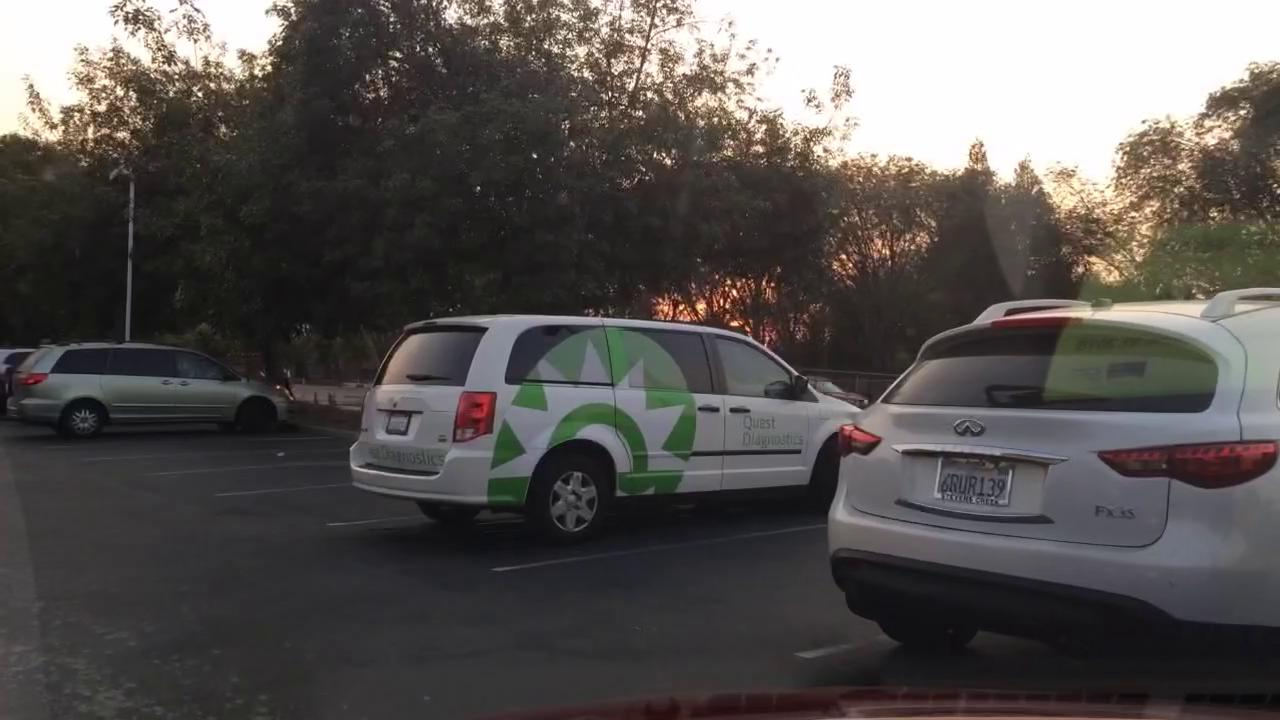
\includegraphics[width=0.31\linewidth]{images/bdd100k_samples/img1.jpg} &
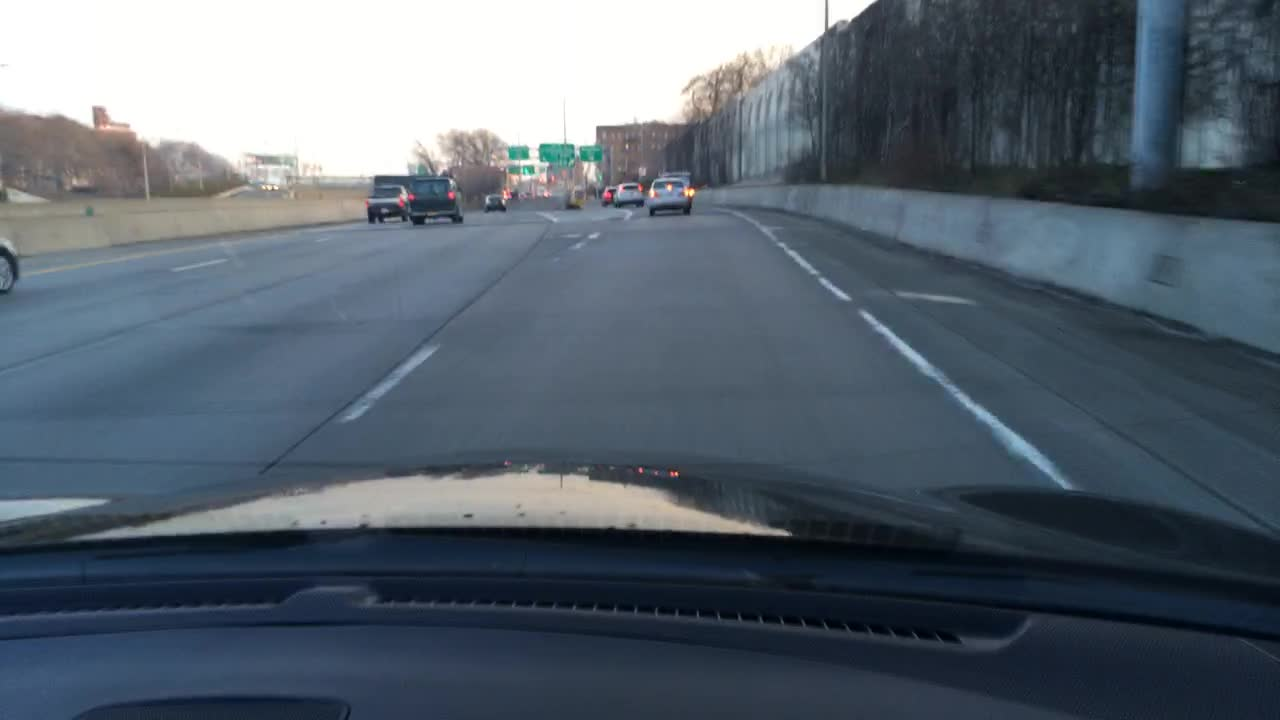
\includegraphics[width=0.31\linewidth]{images/bdd100k_samples/img2.jpg} &
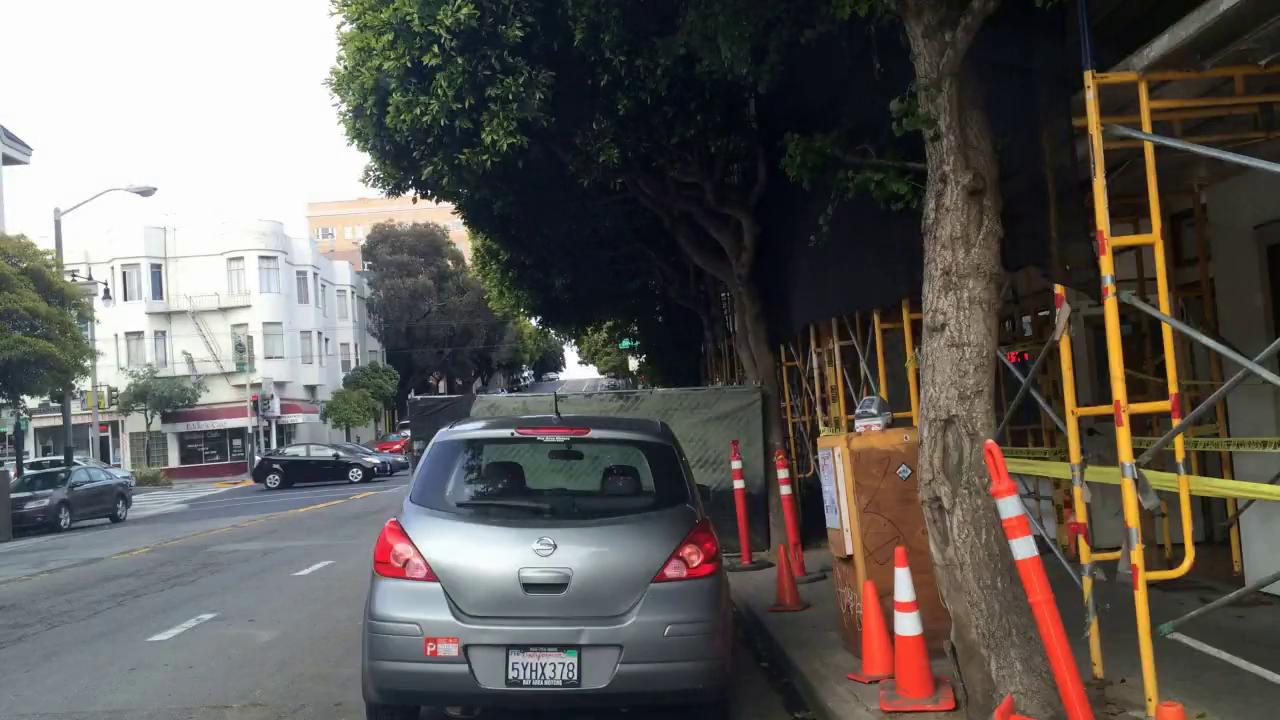
\includegraphics[width=0.31\linewidth]{images/bdd100k_samples/img3.jpg} \\
\small (a) Scene Image 1 & \small (b) Scene Image 2 & \small (c) Scene Image 3 \\[1ex]
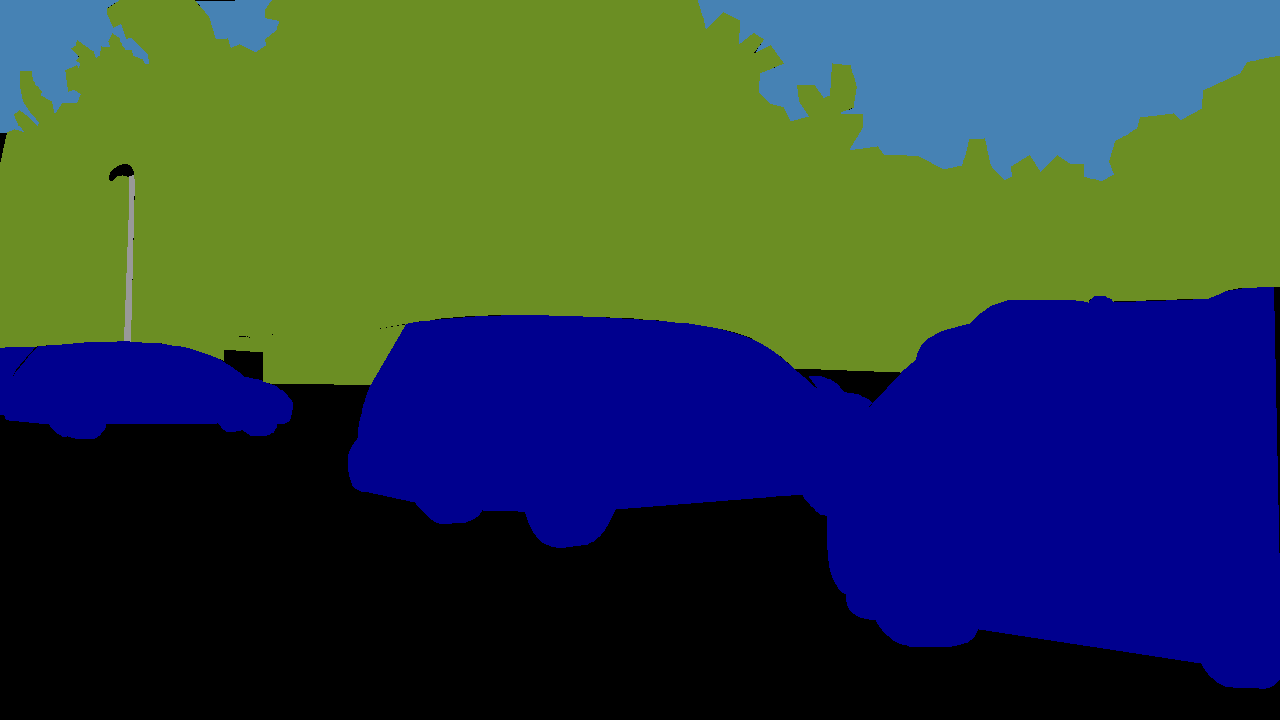
\includegraphics[width=0.31\linewidth]{images/bdd100k_samples/mask1.png} &
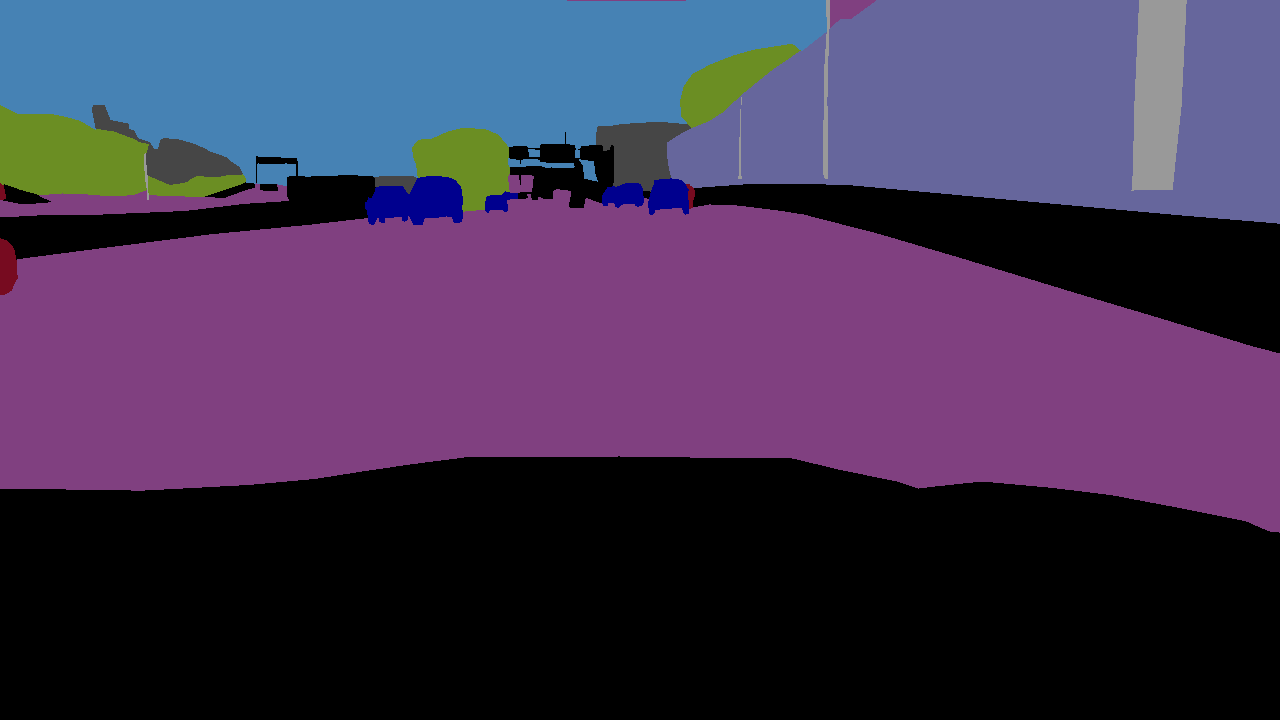
\includegraphics[width=0.31\linewidth]{images/bdd100k_samples/mask2.png} &
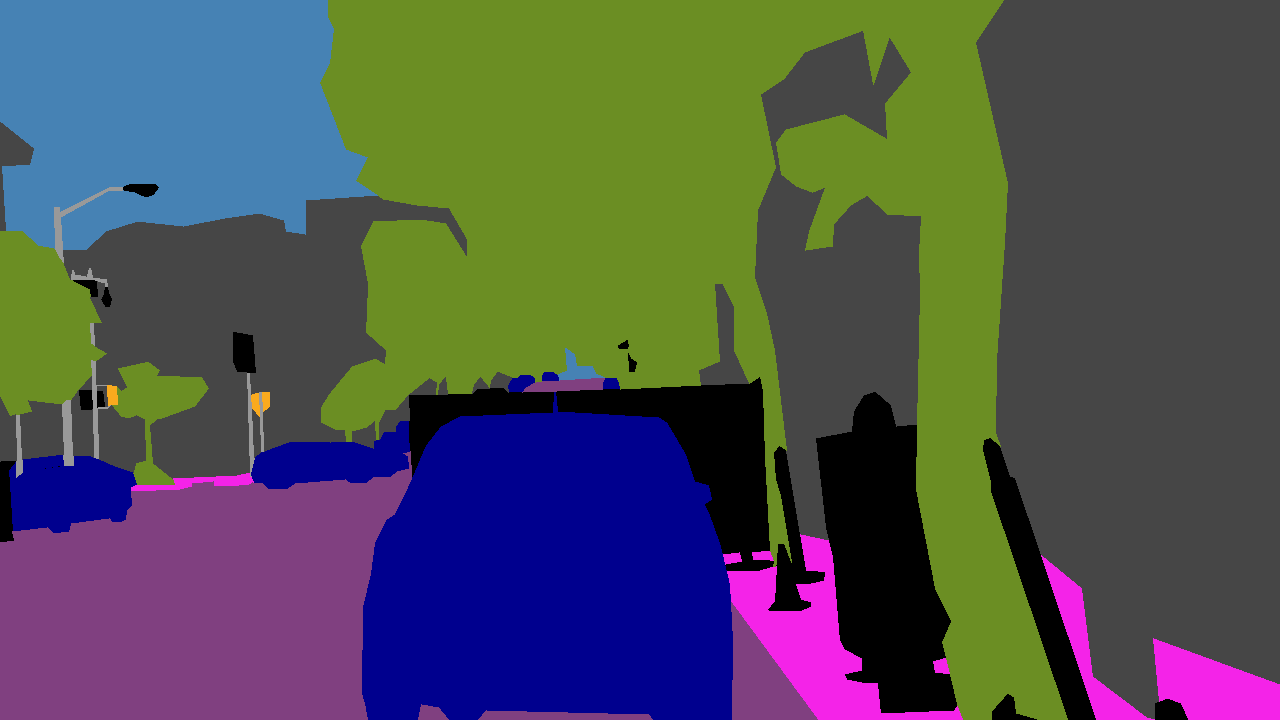
\includegraphics[width=0.31\linewidth]{images/bdd100k_samples/mask3.png} \\
\small (d) Ground Truth 1 & \small (e) Ground Truth 2 & \small (f) Ground Truth 3 \\
\end{tabular}
\caption{Sample $2 \times 3$ grid from the BDD100K dataset: top row shows RGB driving scene images, bottom row shows the corresponding pixel-level ground truth semantic segmentation color labels~\cite{bdd100k2020}.}
\label{fig:bdd100k_grid}
\end{figure}



\chapter{Methodology and Architecture Design}

This chapter details the two KAN-based segmentation architectures: the full-precision UKAN and the binarized BiKASegNet. We describe the integration of KAN layers into the U-Net framework, the design of binarized KAN convolutions, and the knowledge distillation pipeline connecting both models.

\section{UKAN: U-Shaped KAN Segmentation Network}
\label{sec:ukan_arch}
UKAN adapts the U-Net architecture by replacing the standard MLP/Transformer blocks in the bottleneck and lower-resolution stages with KAN-based blocks, while retaining efficient CNN stages at higher resolutions where spatial dimensions are large.

\subsection{Overall Architecture}
The UKAN architecture follows a three-stage CNN encoder, a KAN encoder-bottleneck, and a mixed KAN-CNN decoder, as illustrated in Figure~\ref{fig:ukan_arch}.

\begin{figure}[htbp]
    \centering
    \resizebox{0.95\textwidth}{!}{%
    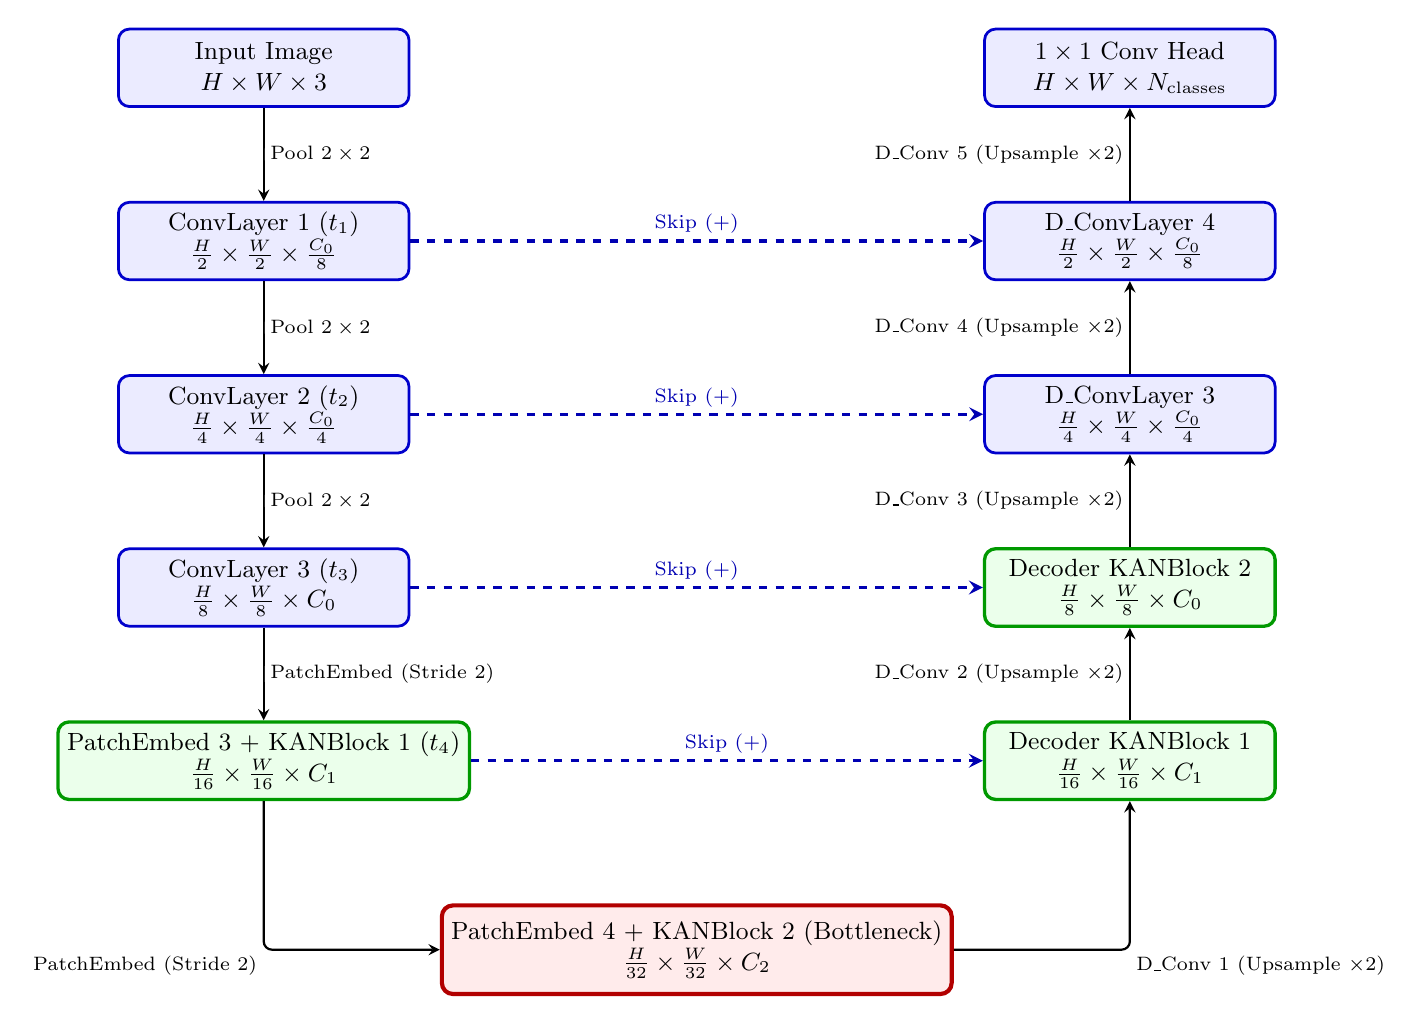
\begin{tikzpicture}[>=stealth, thick]
        \tikzset{
            conv/.style={draw=blue!80!black, fill=blue!8, rectangle, minimum height=2.8em, minimum width=10.5em, rounded corners, align=center, font=\small, line width=1pt},
            kan/.style={draw=green!60!black, fill=green!8, rectangle, minimum height=2.8em, minimum width=10.5em, rounded corners, align=center, font=\small, line width=1.2pt},
            bottleneck/.style={draw=red!70!black, fill=red!8, rectangle, minimum height=3.2em, minimum width=14em, rounded corners, align=center, font=\small, line width=1.5pt},
            io/.style={font=\scriptsize, align=center, fill=white, inner sep=2pt},
            line/.style={draw, ->, >=stealth, thick, rounded corners=3pt},
            skipline/.style={draw, ->, >=stealth, dashed, blue!70!black, line width=1.2pt}
        }
        
        % Left Side (Encoder - Downsampling Path)
        \node[conv] (input) at (0, 0) {Input Image\\$H \times W \times 3$};
        \node[conv] (e1) at (0, -2.2) {ConvLayer 1 ($t_1$)\\$\frac{H}{2} \times \frac{W}{2} \times \frac{C_0}{8}$};
        \node[conv] (e2) at (0, -4.4) {ConvLayer 2 ($t_2$)\\$\frac{H}{4} \times \frac{W}{4} \times \frac{C_0}{4}$};
        \node[conv] (e3) at (0, -6.6) {ConvLayer 3 ($t_3$)\\$\frac{H}{8} \times \frac{W}{8} \times C_0$};
        \node[kan] (e4) at (0, -8.8) {PatchEmbed 3 $+$ KANBlock 1 ($t_4$)\\$\frac{H}{16} \times \frac{W}{16} \times C_1$};
        
        % Bottom Center (Bottleneck)
        \node[bottleneck] (b) at (5.5, -11.2) {PatchEmbed 4 $+$ KANBlock 2 (Bottleneck)\\$\frac{H}{32} \times \frac{W}{32} \times C_2$};
        
        % Right Side (Decoder - Upsampling Path)
        \node[kan] (d4) at (11, -8.8) {Decoder KANBlock 1\\$\frac{H}{16} \times \frac{W}{16} \times C_1$};
        \node[kan] (d3) at (11, -6.6) {Decoder KANBlock 2\\$\frac{H}{8} \times \frac{W}{8} \times C_0$};
        \node[conv] (d2) at (11, -4.4) {D\_ConvLayer 3\\$\frac{H}{4} \times \frac{W}{4} \times \frac{C_0}{4}$};
        \node[conv] (d1) at (11, -2.2) {D\_ConvLayer 4\\$\frac{H}{2} \times \frac{W}{2} \times \frac{C_0}{8}$};
        \node[conv] (final) at (11, 0) {$1\times1$ Conv Head\\$H \times W \times N_{\text{classes}}$};
        
        % Downsampling Connections (Encoder)
        \path[line] (input) -- node[right, io] {Pool $2\times2$} (e1);
        \path[line] (e1) -- node[right, io] {Pool $2\times2$} (e2);
        \path[line] (e2) -- node[right, io] {Pool $2\times2$} (e3);
        \path[line] (e3) -- node[right, io] {PatchEmbed (Stride 2)} (e4);
        \path[line] (e4) |- node[below left, io] {PatchEmbed (Stride 2)} (b.west);
        
        % Upsampling Connections (Decoder)
        \path[line] (b.east) -| node[below right, io] {D\_Conv 1 (Upsample $\times2$)} (d4);
        \path[line] (d4) -- node[left, io] {D\_Conv 2 (Upsample $\times2$)} (d3);
        \path[line] (d3) -- node[left, io] {D\_Conv 3 (Upsample $\times2$)} (d2);
        \path[line] (d2) -- node[left, io] {D\_Conv 4 (Upsample $\times2$)} (d1);
        \path[line] (d1) -- node[left, io] {D\_Conv 5 (Upsample $\times2$)} (final);
        
        % Horizontal Skip Connections across the U-Shape
        \path[skipline] (e1) -- node[above, io] {Skip ($+$)} (d1);
        \path[skipline] (e2) -- node[above, io] {Skip ($+$)} (d2);
        \path[skipline] (e3) -- node[above, io] {Skip ($+$)} (d3);
        \path[skipline] (e4) -- node[above, io] {Skip ($+$)} (d4);
        
    \end{tikzpicture}
    }
    \vspace{1ex}
    
    {\small \textit{*Note: Green blocks indicate KAN-based stages. Blue blocks indicate standard CNN stages. Red block indicates the KAN bottleneck. Dashed lines indicate horizontal skip connections across the U-shape.}}
    \caption{UKAN Architecture: Symmetric U-shaped encoder-decoder network transitioning from CNN stages to KAN blocks at lower resolutions, connected by horizontal skip connections.}
    \label{fig:ukan_arch}
\end{figure}

The encoder consists of three CNN stages (ConvLayer), each performing a double $3\times3$ convolution with BatchNorm and ReLU, followed by $2\times2$ max pooling. The channel dimensions progress as $3 \rightarrow C_0/8 \rightarrow C_0/4 \rightarrow C_0$, where $C_0$ is the base embedding dimension (default: 64).

\subsection{KAN Encoder and Bottleneck}
At the transition from CNN to KAN stages, PatchEmbed layers convert 2D feature maps into 1D token sequences via a strided convolution projection:
\begin{equation}
    \mathbf{T} = \text{LayerNorm}\left(\text{reshape}\left(\text{Conv}_{k \times k, s}(\mathbf{F})\right)\right) \in \mathbb{R}^{B \times N \times C}
\end{equation}
where $\mathbf{F}$ is the input feature map, $k$ is the patch size, $s$ is the stride, and $N = H' \times W'$ is the number of tokens. Two KAN encoder stages process tokens at embedding dimensions $C_1 = 128$ and $C_2 = 256$ (default configuration).

\subsection{KANBlock Design}
Each KANBlock follows a Transformer-style pre-norm residual pattern:
\begin{equation}
    \mathbf{T}' = \mathbf{T} + \text{DropPath}\left(\text{KANLayer}(\text{LayerNorm}(\mathbf{T}), H, W)\right)
\end{equation}
The KANLayer replaces the standard MLP (or self-attention) module. It consists of three KAN linear projections interleaved with depthwise convolution blocks (DW\_bn\_relu) for spatial token mixing:
\begin{align}
    \mathbf{T}_1 &= \text{DW\_bn\_relu}\left(\text{KAN\_fc}_1(\mathbf{T}), H, W\right) \\
    \mathbf{T}_2 &= \text{DW\_bn\_relu}\left(\text{KAN\_fc}_2(\mathbf{T}_1), H, W\right) \\
    \mathbf{T}_3 &= \text{DW\_bn\_relu}\left(\text{KAN\_fc}_3(\mathbf{T}_2), H, W\right)
\end{align}
Each KAN\_fc is an instance of the selected KAN linear variant (FasterKAN, ReLU-KAN, etc.) with grid size $G=8$. The depthwise convolutions preserve spatial context since KAN operations act independently on the channel dimension. Each DW\_bn\_relu block performs:
\begin{equation}
    \text{DW\_bn\_relu}(\mathbf{T}, H, W) = \text{ReLU}\left(\text{BN}\left(\text{DWConv}_{3\times3}(\text{reshape}(\mathbf{T}, H, W))\right)\right)
\end{equation}

\subsection{KAN Variant Layer Integration in UKAN}
\label{sec:kan_variant_integration}
While Chapter~\ref{ch:background} described the mathematical definitions and linearity properties of the individual activation functions, this section details how HardSwish-KAN, TeLU-KAN, and PWLO-KAN are parameterized as edge-centric linear projection layers within the UKAN architecture.

\subsubsection{HardSwish-KAN Linear Layer}
HardSwish-KAN integrates the piecewise-linear HardSwish activation into the KAN grid expansion. For an input vector $\mathbf{x} \in \mathbb{R}^{d_{\text{in}}}$, LayerNorm is first applied. A uniform grid of knot points $\{g_0, \dots, g_{G-1}\}$ is constructed across $[g_{\min}, g_{\max}]$. Each feature $x_i$ is evaluated against all grid offsets:
\begin{equation}
    \psi_k(x_i) = \text{HardSwish}(x_i - g_k) = (x_i - g_k) \cdot \frac{\text{ReLU6}(x_i - g_k + 3)}{6}
\end{equation}
The evaluations from all $G$ knot points across $d_{\text{in}}$ dimensions are concatenated into $\text{vec}\left(\{\psi_k(x_i)\}\right) \in \mathbb{R}^{d_{\text{in}} \cdot G}$ and projected via a learnable weight matrix $\mathbf{W} \in \mathbb{R}^{d_{\text{out}} \times (d_{\text{in}} \cdot G)}$.

\subsubsection{TeLU-KAN Linear Layer}
TeLU-KAN constructs edge-centric transformations by applying the TeLU function over grid-shifted inputs:
\begin{equation}
    \psi_k(x_i) = \text{TeLU}(x_i - g_k) = (x_i - g_k) \cdot \tanh(\exp(x_i - g_k))
\end{equation}
The resulting basis evaluations are concatenated and linearly projected via $\mathbf{W} \in \mathbb{R}^{d_{\text{out}} \times (d_{\text{in}} \cdot G)}$. This leverages TeLU's identity-like positive region linearity to provide unattenuated gradient propagation across deep KAN blocks.

\subsubsection{PWLO-KAN Linear Layer}
PWLO-KAN implements an explicit lookup-table (LUT) structure for high-efficiency integer and edge inference. Given domain bounds $[g_{\min}, g_{\max}]$ and segment count $G$, the interval step size is $\Delta = \frac{g_{\max} - g_{\min}}{G}$. For each input feature $x_i$, the active segment index $k$ is determined via clamped index quantization:
\begin{equation}
    k = \text{clamp}\left(\left\lfloor \frac{x_i - g_{\min}}{\Delta} \right\rfloor, 0, G-1\right)
\end{equation}
Rather than evaluating continuous functions, PWLO-KAN retrieves learned affine parameters $a_{i,k}$ and $b_{i,k}$ from embedding tables $\mathbf{A}, \mathbf{B} \in \mathbb{R}^{(d_{\text{in}} \cdot G) \times d_{\text{out}}}$ to evaluate localized affine transformations $\phi_k(x_i) = a_{i,k} \cdot x_i + b_{i,k}$. This enables the entire layer to execute via fast table lookups and linear shift-and-add operations.

\subsection{Decoder}
The decoder combines KAN blocks with standard convolutional upsampling (D\_ConvLayer). Each decoder stage: (1) applies a D\_ConvLayer convolution to reduce channels, (2) bilinearly upsamples by factor 2, (3) adds the skip connection from the corresponding encoder stage, (4) processes with a decoder KANBlock. The final three stages use only D\_ConvLayers to restore the original spatial resolution, followed by a $1\times1$ convolution head producing per-class logits.


\section{BiKASegNet: Binarized KAN Segmentation Network}
\label{sec:bika_arch}
BiKASegNet implements the KAN philosophy of learnable per-connection activations in a radically different way: instead of smooth spline functions, it uses binarized step functions with learnable per-connection thresholds. This produces a network where both weights and activations are binary ($\{+1, -1\}$), enabling extreme computational efficiency.

\subsection{Adapting BiKA Layers for Semantic Road Segmentation}
\label{sec:bika_adapting_layers}
While Section~\ref{sec:bika_conv2d} defined the theoretical formulation of the \texttt{BiKA\_Conv2d} binarized layer, adapting 1-bit per-connection activation layers for dense semantic road segmentation requires structural and channel-capacity modifications to overcome severe quantization loss and maintain stable gradient propagation across deep networks.

\subsubsection{Overall Architectural Adaptation \& Channel Width Scaling}
To transition BiKA from classification tasks to dense pixel-wise segmentation on high-resolution driving datasets (e.g., BDD100K), an overall architectural adaptation was developed by constructing a U-Net style encoder-decoder network around binarized blocks. In this framework, channel capacity plays a critical role in balancing model expressiveness with hardware efficiency. Two primary channel width scaling configurations were developed and evaluated in the \texttt{BiKA} repository:

\begin{itemize}
    \item \textbf{16-Channel Baseline Configuration (\texttt{base\_channels = 16})}:
    In this ultra-lightweight setup, channel dimensions progress across encoder stages as $C \rightarrow 2C \rightarrow 4C \rightarrow 8C$, corresponding to $16 \rightarrow 32 \rightarrow 64 \rightarrow 128$ channels. This model contains only $\sim$0.35M parameters with an extremely small memory footprint ($\sim$1.4\,MB). It is specifically engineered for sub-watt microcontrollers and embedded FPGAs where memory bandwidth and cache capacities are severely constrained.
    
    \item \textbf{32-Channel Capacity Update (\texttt{base\_channels = 32})}:
    To match the parameter capacity ($\sim$4.1M parameters) and representational bandwidth of full-precision baseline networks (such as UKAN), the network architecture was updated to use a base channel count of $C = 32$. Here, stage channels expand as $32 \rightarrow 64 \rightarrow 128 \rightarrow 256$. Doubling the base channel width quadruples the binary feature interaction capacity across layers, enabling the network to resolve subtle spatial boundaries, thin lane markings, and distant road obstacles with significantly higher segmentation mIoU, while retaining 100\% multiply-free bitwise XNOR and popcount acceleration during inference.
\end{itemize}

\subsubsection{Full-Precision FP32 Stem (\texttt{full\_precision\_stem})}
The initial input stage (\texttt{self.enc1}) processes raw RGB images ($3 \times H \times W$) using a full-precision $3\times3$ FP32 convolution projection ($3 \rightarrow C$), followed by BatchNorm and RPReLU, before passing features to \texttt{BiKA\_Conv2d}. Direct binarization of continuous 8-bit RGB pixel values at the input layer severely degrades spatial details and accuracy, as raw pixel intensities lack the high-dimensional channel representation required for effective 1-bit thresholding.

\subsubsection{ReActNet-Inspired RPReLU Activations}
Standard ReLU activations set all negative values to zero ($\max(0, x)$), which leads to severe information loss and dead neurons in binary networks. BiKASegNet replaces standard ReLU with ReActNet-style RPReLU (Re-Activation PReLU):
\begin{equation}
    \text{RPReLU}(x) = \text{PReLU}(x + \gamma) + \beta
\end{equation}
where $\gamma, \beta \in \mathbb{R}^{1 \times C \times 1 \times 1}$ are learnable per-channel pre-shift and post-shift parameters. RPReLU dynamically shifts binary activation distributions before and after non-linearities, allowing asymmetric activation ranges necessary for fine-grained pixel-wise road classification.

\subsubsection{Full-Precision FP32 Classification Head (\texttt{full\_precision\_head})}
The final segmentation output layer (\texttt{self.final}) uses a $1\times1$ FP32 convolution projection ($C \rightarrow N_{\text{classes}}$) rather than a binary convolution. Retaining full-precision weights and biases at the final layer ensures smooth, continuous logit distributions, which are essential for computing precise pixel-wise Cross-Entropy and Dice loss gradients during backpropagation.

\subsubsection{Feature Concatenation in U-Net Decoder}
Unlike additive skip connections, the BiKASegNet decoder concatenates encoder skip features with upsampled decoder features ($\text{dec3}$ takes $8C + 4C = 12C$ channels to $4C$, $\text{dec2}$ takes $4C + 2C = 6C$ channels to $2C$, and $\text{dec1}$ takes $2C + C = 3C$ channels to $C$). Feature concatenation preserves independent binary feature channels across spatial resolutions, providing richer representation recombination for multi-scale road and lane boundary segmentations.

\subsection{BiKAConvBlock Design}
Each \texttt{BiKAConvBlock} integrates two \texttt{BiKA\_Conv2d} layers with BatchNorm, RPReLU activations, and an FP32 shortcut connection (Bi-Real Net style):
\begin{align}
    \mathbf{s} &= \text{Shortcut}(\mathbf{x}) \\
    \mathbf{h} &= \text{RPReLU}\left(\text{BN}\left(\text{BiKA\_Conv2d}_1(\mathbf{x})\right)\right) \\
    \mathbf{y} &= \text{RPReLU}\left(\text{BN}\left(\text{BiKA\_Conv2d}_2(\mathbf{h})\right) + \mathbf{s}\right)
\end{align}
The shortcut $\text{Shortcut}(\mathbf{x})$ is a $1\times1$ FP32 convolution with BatchNorm when channel dimensions change, and an identity mapping otherwise. To manage memory consumption during training, activation checkpointing (\texttt{torch.utils.checkpoint}) is applied to \texttt{BiKAConvBlock}, reducing peak GPU VRAM usage by approximately 60\%.

\subsection{BiKASegNet Architecture}
The full BiKASegNet follows a standard U-Net topology with BiKAConvBlocks replacing standard convolution blocks, as shown in Figure~\ref{fig:bika_arch}.

\begin{figure}[htbp]
\centering
\resizebox{0.95\textwidth}{!}{%
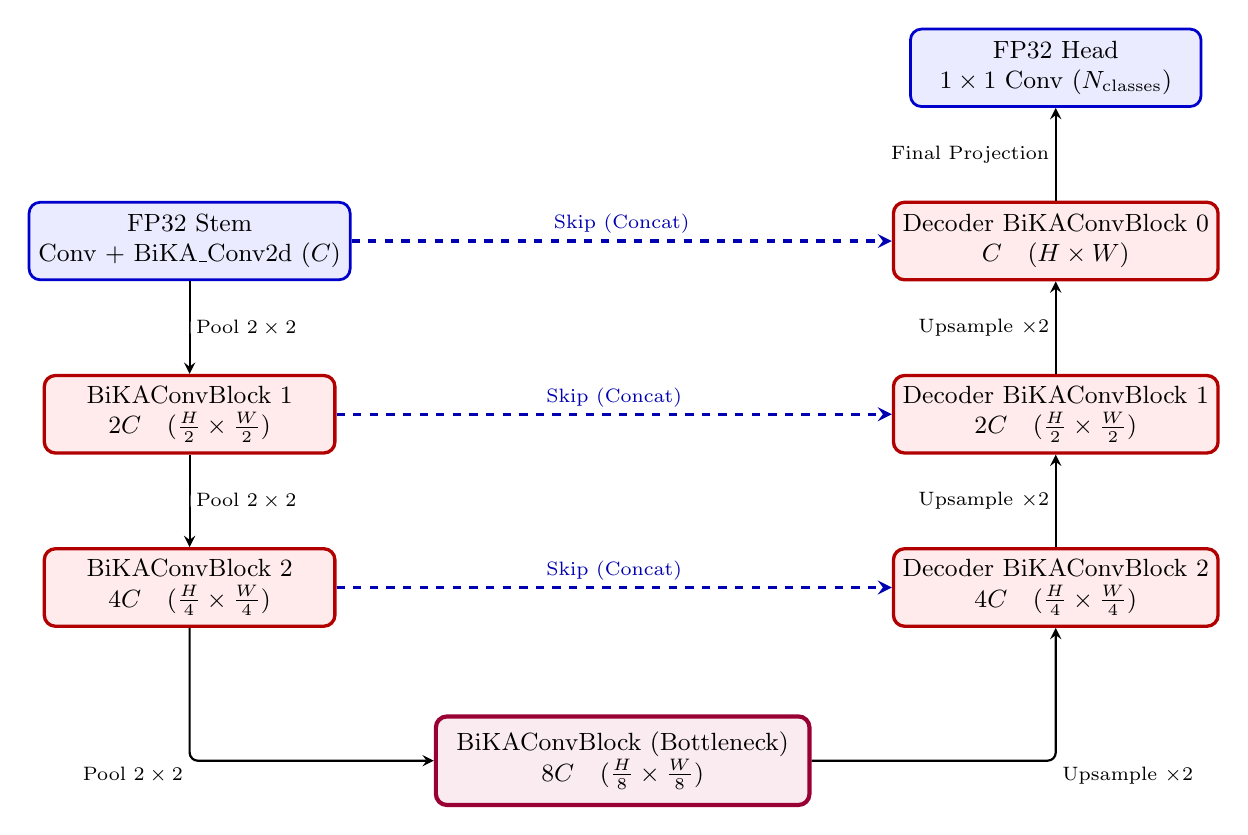
\begin{tikzpicture}[>=stealth, thick]
    \tikzset{
        fp/.style={draw=blue!80!black, fill=blue!8, rectangle, minimum height=2.8em, minimum width=10.5em, rounded corners, align=center, font=\small, line width=1pt},
        bin/.style={draw=red!70!black, fill=red!8, rectangle, minimum height=2.8em, minimum width=10.5em, rounded corners, align=center, font=\small, line width=1.2pt},
        bottleneck/.style={draw=purple!80!black, fill=purple!8, rectangle, minimum height=3.2em, minimum width=13.5em, rounded corners, align=center, font=\small, line width=1.5pt},
        io/.style={font=\scriptsize, align=center, fill=white, inner sep=2pt},
        line/.style={draw, ->, >=stealth, thick, rounded corners=3pt},
        skipline/.style={draw, ->, >=stealth, dashed, blue!70!black, line width=1.2pt}
    }
    
    % Left Side (Encoder - Downsampling Path)
    \node[fp] (stem) at (0, 0) {FP32 Stem\\Conv $+$ BiKA\_Conv2d ($C$)};
    \node[bin] (e2) at (0, -2.2) {BiKAConvBlock 1\\$2C \quad (\frac{H}{2} \times \frac{W}{2})$};
    \node[bin] (e3) at (0, -4.4) {BiKAConvBlock 2\\$4C \quad (\frac{H}{4} \times \frac{W}{4})$};
    
    % Bottom Center (Bottleneck)
    \node[bottleneck] (b) at (5.5, -6.6) {BiKAConvBlock (Bottleneck)\\$8C \quad (\frac{H}{8} \times \frac{W}{8})$};
    
    % Right Side (Decoder - Upsampling Path)
    \node[bin] (d3) at (11, -4.4) {Decoder BiKAConvBlock 2\\$4C \quad (\frac{H}{4} \times \frac{W}{4})$};
    \node[bin] (d2) at (11, -2.2) {Decoder BiKAConvBlock 1\\$2C \quad (\frac{H}{2} \times \frac{W}{2})$};
    \node[bin] (d1) at (11, 0) {Decoder BiKAConvBlock 0\\$C \quad (H \times W)$};
    \node[fp] (head) at (11, 2.2) {FP32 Head\\$1\times1$ Conv ($N_{\text{classes}}$)};
    
    % Downsampling Connections (Encoder)
    \path[line] (stem) -- node[right, io] {Pool $2\times2$} (e2);
    \path[line] (e2) -- node[right, io] {Pool $2\times2$} (e3);
    \path[line] (e3) |- node[below left, io] {Pool $2\times2$} (b.west);
    
    % Upsampling Connections (Decoder)
    \path[line] (b.east) -| node[below right, io] {Upsample $\times 2$} (d3);
    \path[line] (d3) -- node[left, io] {Upsample $\times 2$} (d2);
    \path[line] (d2) -- node[left, io] {Upsample $\times 2$} (d1);
    \path[line] (d1) -- node[left, io] {Final Projection} (head);
    
    % Horizontal Concatenation Skip Connections across the U-Shape
    \path[skipline] (stem) -- node[above, io] {Skip (Concat)} (d1);
    \path[skipline] (e2) -- node[above, io] {Skip (Concat)} (d2);
    \path[skipline] (e3) -- node[above, io] {Skip (Concat)} (d3);
    
\end{tikzpicture}
}
\vspace{1ex}

{\small \textit{*Note: Red blocks indicate binarized BiKA\_Conv2d layers. Blue blocks indicate full-precision FP32 stem and head. Purple block indicates the binary bottleneck. Dashed lines indicate horizontal feature concatenation skip connections across the U-shape.}}
\caption{BiKASegNet Architecture: Symmetric U-shaped binarized encoder-decoder network using BiKAConvBlocks, connected by feature concatenation skip connections.}
\label{fig:bika_arch}
\end{figure}

Key architectural decisions:
\begin{itemize}
    \item \textbf{Full-precision stem}: The first encoder layer uses a standard FP32 convolution for the initial $3 \rightarrow C$ projection, followed by a BiKA\_Conv2d. Binarizing the very first layer severely degrades accuracy since it directly quantizes the raw 8-bit RGB pixel values.
    \item \textbf{Full-precision head}: The final $1\times1$ classification convolution remains in FP32 to preserve the fine-grained logit distributions needed for accurate per-pixel classification.
    \item \textbf{Concatenation skip connections}: Unlike UKAN's additive skips, BiKASegNet concatenates encoder and decoder features before each decoder block, providing richer feature recombination.
    \item \textbf{Base channels}: The default base channel count is $C = 16$, keeping the binary model extremely lightweight.
\end{itemize}




\section{Training Methodology}
\label{sec:training}
\subsection{Optimisation for BNN Stability}
Training BiKASegNet requires careful handling of the binary weight dynamics. Specifically:
\begin{itemize}
    \item \textbf{Weight decay exclusion}: Weight decay is explicitly disabled for all BiKA\_Conv2d parameters (weights and per-connection biases), BatchNorm affine parameters, and RPReLU shift parameters. Applying weight decay to binary thresholds causes them to collapse toward zero, annihilating the STE gradient and killing the backward pass entirely.
    \item \textbf{STE weight clamping}: Binary weights are optionally clamped to $[-1, 1]$ after each optimiser step to ensure they remain within the STE gradient window.
    \item \textbf{Bias initialisation}: Per-connection biases are uniformly initialized in $[-2.0, 0.5]$ to ensure diverse initial activation thresholds across connections.
\end{itemize}

\subsection{Data Augmentation}
Both UKAN and BiKA training pipelines employ the following augmentations via the Albumentations library:
\begin{itemize}
    \item Random horizontal flip (probability 0.5).
    \item Random 90-degree rotation.
    \item CutMix augmentation for regularisation.
    \item Resize to the target input resolution (default: $256 \times 256$ or $512 \times 512$).
    \item ImageNet-standard normalisation ($\mu = [0.485, 0.456, 0.406]$, $\sigma = [0.229, 0.224, 0.225]$).
\end{itemize}

\subsection{Training Infrastructure}
Models are trained using PyTorch with Automatic Mixed Precision (AMP) for memory efficiency (FP16/BF16 forward pass with FP32 master weights). Multi-GPU training is supported via Distributed Data Parallel (DDP) with \texttt{torchrun}. Learning rate scheduling uses CosineAnnealingLR or OneCycleLR, and gradient accumulation is available for simulating larger effective batch sizes.



\chapter{Experimental Evaluation and Results}

This chapter details the experimental setup, dataset preparation, and performance evaluation of UKAN and BiKASegNet on the BDD100K road segmentation benchmark.

\section{Experimental Setup}
All experiments were conducted on a Linux workstation equipped with NVIDIA GPUs. The software stack consists of Python 3.10, PyTorch 2.x, and the Albumentations augmentation library. Models were trained on the BDD100K dataset~\cite{bdd100k2020}, which provides densely annotated driving scene images with per-pixel semantic labels covering road surfaces, lane markings, vehicles, pedestrians, and background categories. We evaluate in both a 2-class configuration (road foreground vs. background) and the full multi-class configuration.

\section{Segmentation Quality Benchmarks}
\label{sec:seg_benchmarks}

The primary evaluation metrics are mean Intersection over Union (mIoU) and mean Dice coefficient, computed via a confusion-matrix-based epoch-level accumulator to avoid batch-averaging inaccuracies.

The IoU for class $c$ is computed as:
\begin{equation}
    \text{IoU}_c = \frac{\text{TP}_c}{\text{TP}_c + \text{FP}_c + \text{FN}_c}
\end{equation}
and the Dice coefficient as:
\begin{equation}
    \text{Dice}_c = \frac{2 \cdot \text{TP}_c}{2 \cdot \text{TP}_c + \text{FP}_c + \text{FN}_c}
\end{equation}
where $\text{TP}_c$, $\text{FP}_c$, and $\text{FN}_c$ are the true positives, false positives, and false negatives for class $c$ accumulated over the entire validation set.

Table~\ref{tab:segmentation_results} summarizes the segmentation performance of the evaluated architectures.

\begin{table}[h!]
\centering
\begin{tabular}{lcccc}
\toprule
\textbf{Model} & \textbf{Precision} & \textbf{KAN Variant} & \textbf{mIoU (\%)} & \textbf{Dice (\%)} \\
\midrule
U-Net (Baseline) & FP32 & -- & -- & -- \\
UKAN (FasterKAN) & FP32 & RSWAf & -- & -- \\
UKAN (ReLU-KAN) & FP32 & ReLU & -- & -- \\
UKAN (PWLO-KAN) & FP32 & PWLO & -- & -- \\
BiKASegNet & 1-bit & Binary Step & -- & -- \\
BiKASegNet + KD & 1-bit & Binary Step & -- & -- \\
\bottomrule
\end{tabular}
\vspace{1ex}

{\small \textit{*Note: Results to be filled from experimental runs. KD = Knowledge Distillation from UKAN teacher.}}
\caption{Segmentation accuracy comparison across architectures on BDD100K road segmentation.}
\label{tab:segmentation_results}
\end{table}


\section{Model Efficiency Analysis}
\label{sec:efficiency}

Table~\ref{tab:efficiency_results} compares the model size and computational efficiency of the evaluated architectures.

\begin{table}[h!]
\centering
\begin{tabular}{lcccc}
\toprule
\textbf{Model} & \textbf{Params (M)} & \textbf{Size (MB)} & \textbf{FPS} & \textbf{Compression} \\
\midrule
U-Net (FP32) & -- & -- & -- & $1\times$ \\
UKAN (FP32) & -- & -- & -- & $1\times$ \\
BiKASegNet (1-bit) & -- & -- & -- & $\sim32\times$ \\
\bottomrule
\end{tabular}
\vspace{1ex}

{\small \textit{*Note: Compression ratio is relative to the FP32 model of equivalent architecture. FPS measured on the evaluation GPU.}}
\caption{Model efficiency comparison: parameter count, storage size, inference throughput, and compression ratio.}
\label{tab:efficiency_results}
\end{table}

The theoretical compression ratio of BiKASegNet relative to a full-precision network of identical topology is approximately $32\times$ for the binarized layers, since each 32-bit float weight is replaced by a single bit. In practice, the full-precision stem and head slightly reduce the overall compression ratio.

\subsection{Inference Throughput}
The binary convolution operations in BiKA\_Conv2d leverage XNOR and popcount operations through the custom CUDA kernel. Table~\ref{tab:latency_profile} profiles the per-layer latency contributions.

\begin{table}[h!]
\centering
\begin{tabular}{lcc}
\toprule
\textbf{Component} & \textbf{UKAN Latency (ms)} & \textbf{BiKA Latency (ms)} \\
\midrule
Encoder Stages       & -- & -- \\
KAN/Binary Blocks    & -- & -- \\
Decoder Stages       & -- & -- \\
Classification Head  & -- & -- \\
\midrule
\textbf{Total}       & -- & -- \\
\bottomrule
\end{tabular}
\vspace{1ex}

{\small \textit{*Note: Latency measured as mean over 1000 forward passes at $512 \times 512$ input resolution.}}
\caption{Per-component inference latency comparison between UKAN and BiKASegNet.}
\label{tab:latency_profile}
\end{table}


\section{Ablation Studies}
\label{sec:ablations}

\subsection{Effect of KAN Variant Selection}
To isolate the impact of the KAN activation function choice, we trained UKAN with each variant using identical hyperparameters. The KAN variant selection affects both accuracy and inference speed, as each variant trades off the smoothness of the learned activation against computational cost.

\subsection{Effect of Knowledge Distillation}
Table~\ref{tab:kd_ablation} examines the impact of knowledge distillation on BiKASegNet accuracy.

\begin{table}[h!]
\centering
\begin{tabular}{lccc}
\toprule
\textbf{Configuration} & \textbf{Teacher} & \textbf{mIoU (\%)} & \textbf{$\Delta$ mIoU} \\
\midrule
BiKA (no KD) & -- & -- & -- \\
BiKA + KD ($\tau=4$) & UKAN-FasterKAN & -- & -- \\
BiKA + KD + Boundary & UKAN-FasterKAN & -- & -- \\
\bottomrule
\end{tabular}
\vspace{1ex}

{\small \textit{*Note: $\Delta$ mIoU is relative to the no-KD baseline.}}
\caption{Ablation study on knowledge distillation and boundary loss for BiKASegNet.}
\label{tab:kd_ablation}
\end{table}

\subsection{Effect of BNN Training Techniques}
We evaluate the individual contribution of each BNN accuracy-improvement technique integrated into BiKAConvBlock:
\begin{itemize}
    \item \textbf{Libra-PB}: Weight centering for balanced binarization.
    \item \textbf{RPReLU}: Learnable activation shifts vs. standard ReLU.
    \item \textbf{FP32 Skip}: Bi-Real Net gradient highway connections.
    \item \textbf{AdaBin}: Learnable output scaling.
\end{itemize}
Disabling the legacy mode activates all four techniques simultaneously. In legacy mode, the network reverts to plain ReLU activations and no skip connections, establishing the minimal BNN baseline.



\chapter{Conclusions and Future Works}

\section{Conclusions}
In this thesis, we implemented, evaluated, and compared two complementary approaches for integrating Kolmogorov-Arnold Networks into segmentation architectures for road scene understanding.

The UKAN architecture demonstrates that replacing standard MLP projections with KAN layers in the U-Net bottleneck produces competitive segmentation quality while offering greater representational flexibility through learnable per-edge activation functions. The availability of multiple KAN variants (FasterKAN, ReLU-KAN, HardSwish-KAN, PWLO-KAN, TeLU-KAN) enables architecture-level tuning of the accuracy-latency trade-off depending on the deployment target.

The BiKASegNet architecture demonstrates that the KAN philosophy of per-connection learnable activations can be realized through binarized step functions with learnable thresholds, achieving extreme compression ($\sim$32$\times$) and computational acceleration through XNOR/popcount operations. The integration of state-of-the-art BNN techniques (Libra-PB, AdaBin, RPReLU, FP32 skip connections) is essential for maintaining segmentation quality under binary constraints. Knowledge distillation from a full-precision UKAN teacher further bridges the binarization gap.

\section{Future Works}
To extend this research, several areas should be investigated:
\begin{itemize}
    \item \textbf{Edge Deployment}: Deploy BiKASegNet on actual embedded platforms (Raspberry Pi, Jetson Nano) and benchmark real-world inference latency and power consumption.
    \item \textbf{Multi-class Segmentation}: Extend the evaluation from 2-class road segmentation to the full BDD100K label set (20+ classes) and evaluate how KAN integration affects fine-grained category discrimination.
    \item \textbf{Temporal Consistency}: Integrate the segmentation networks into a video pipeline with temporal smoothing to evaluate frame-to-frame consistency of road boundary predictions.
    \item \textbf{Hybrid KAN-BNN Architectures}: Explore architectures that selectively apply binarization only to specific encoder/decoder stages while keeping KAN-critical bottleneck layers in higher precision.
\end{itemize}
\newpage
\nocite{}
\addcontentsline{toc}{chapter}{Bibliography}
\thispagestyle{noNumber}
\bibliographystyle{ieeetr}
\bibliography{references}

\end{document}

